\documentclass[12pt, twoside]{article}
\usepackage[letterpaper, margin=1in, headsep=0.5in]{geometry}
\usepackage[english]{babel}
\usepackage[utf8]{inputenc}
\usepackage{amsmath}
\usepackage{amsfonts}
\usepackage{amssymb}
\usepackage{tikz}
\usetikzlibrary{quotes, angles}
\usepackage{graphicx}
%\usepackage{pgfplots}
%\pgfplotsset{width=10cm,compat=1.9}
%\usepgfplotslibrary{statistics}
%\usepackage{pgfplotstable}
%\usepackage{tkz-fct}
%\usepackage{venndiagram}

\usepackage{fancyhdr}
\pagestyle{fancy}
\fancyhf{}
\renewcommand{\headrulewidth}{0pt} % disable the underline of the header

\fancyhead[RE]{\thepage}
\fancyhead[RO]{\thepage \\ Name: \hspace{3cm}}
\fancyhead[L]{BECA / Dr. Huson / Geometry 10th Grade\\* Unit 3: Volume and angle bisectors \\ 
10 October 2019}

\begin{document}
  \subsubsection*{3.5 Do Now: Modeling angle situations with an equation}
  \begin{enumerate}
    \subsubsection*{Do Not Solve! \\
    Model the situation with an equation. Circle where it states what to find.}
    \vspace{0.5cm}

\item Two lines intersect making four angles: $\angle 1$, $\angle 2$, $\angle 3$, and $\angle 4$. Given that $m\angle 1= 4x+5$ and $m\angle 4=6x+15$, find $x$.
\begin{flushright}
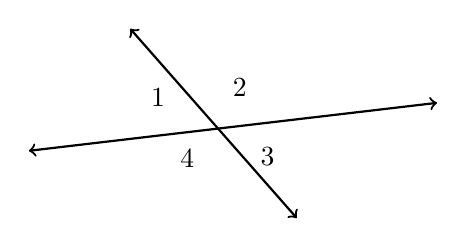
\begin{tikzpicture}[scale=0.5, rotate=-10]
  \draw [<->, thick] (0,-1.5)--(10,1.5);
  \draw [<->, thick] (2,2)--(7,-2);
  \node at (3,.4){1};
  \node at (6,-.6){3};
  \node at (5,1){2};
  \node at (4,-1){4};
\end{tikzpicture}
\end{flushright}

\item Given that $m\angle 2= 5x+8$ and $m\angle 4=7x-6$ as shown in the diagram, find $m\angle 2$.
\begin{flushright}
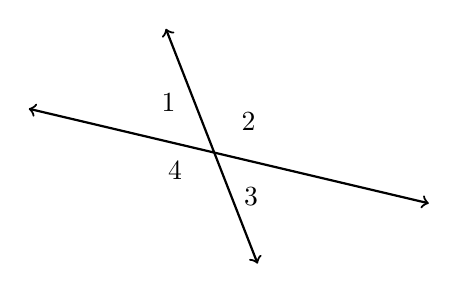
\begin{tikzpicture}[scale=0.5, rotate=-30]
  \draw [<->, thick] (0,-1.5)--(10,1.5);
  \draw [<->, thick] (2,2)--(7,-2);
  \node at (3,.4){1};
  \node at (6,-.6){3};
  \node at (5,1){2};
  \node at (4,-1){4};
\end{tikzpicture}
\end{flushright}

\item In the diagram below $m\angle AOB = 2x+5$ and $m\angle COB = 5x+15$. Find $x$. %\vspace{0.25cm}
  \begin{flushright}
  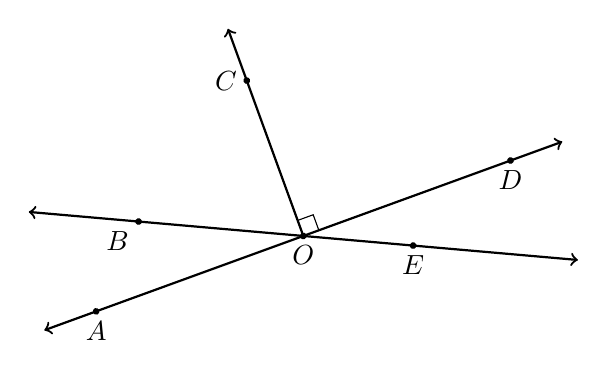
\begin{tikzpicture}[scale=0.7, rotate=20]
    \draw [<->, thick] (-25:5)--(0,0)--(155:5);
    \draw [<->, thick] (-5,0)--(5,0);
    \draw [->, thick] (0,0)--(0,4);
    \draw (0,0)++(0.3,0)--++(0,0.3)--+(-0.3,0);
    %\draw [fill] (-1,2.5) circle [radius=0.05] node[left ]{$B$};
    \draw [fill] (155:3) circle [radius=0.05] node[below left]{$B$};
    \draw [fill] (-4,0) circle [radius=0.05] node[below]{$A$}; 
    \draw [fill] (0,0) circle [radius=0.05] node[below]{$O$};
    \draw [fill] (0,3) circle [radius=0.05] node[left]{$C$};
    \draw [fill] (4,0) circle [radius=0.05] node[below]{$D$};
    \draw [fill] (-25:2) circle [radius=0.05] node[below]{$E$};
  \end{tikzpicture}
  \end{flushright}

  \item In the diagram below $m\angle AOB = 3x+5$, $m\angle BOC = 2x-10$, and $m\angle DOC = x+65^\circ$. Find $m\angle AOB$.
  \begin{flushright}
  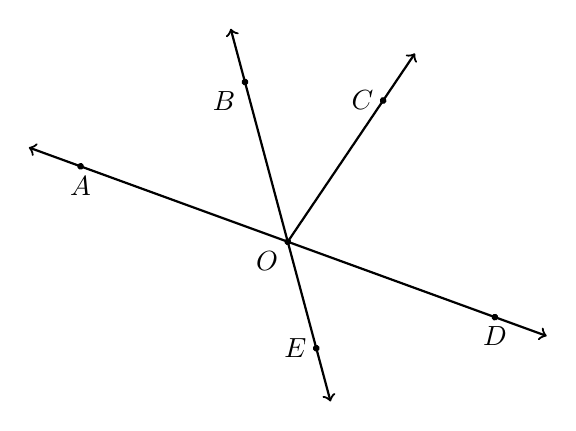
\begin{tikzpicture}[scale=0.7, rotate=-20]
    \draw [<->, thick] (-55:3)--(0,0)--(125:4);
    \draw [<->, thick] (-5,0)--(5,0);
    \draw [->, thick] (0,0)--(1,4);
    %\draw (0,0)++(0.3,0)--++(0,0.3)--+(-0.3,0);
    %\draw [fill] (-1,2.5) circle [radius=0.05] node[left ]{$B$};
    \draw [fill] (125:3) circle [radius=0.05] node[below left]{$B$};
    \draw [fill] (-4,0) circle [radius=0.05] node[below]{$A$}; 
    \draw [fill] (0,0) circle [radius=0.05] node[below left]{$O$};
    \draw [fill] (0.75,3) circle [radius=0.05] node[left]{$C$};
    \draw [fill] (4,0) circle [radius=0.05] node[below]{$D$};
    \draw [fill] (-55:2) circle [radius=0.05] node[left]{$E$};
  \end{tikzpicture}
  \end{flushright}

  \newpage
  \item Complete the construction of the bisector of the given angle. 
  \vspace{1cm}
    \begin{center}
    \begin{tikzpicture}
      \draw [<->, thick] (80:7)--(0,0)--(9,0);
      %\draw [fill] (0,0) circle [radius=0.05] node[below]{$A$};
      %\draw [fill] (5,0) circle [radius=0.05] node[below]{$B$};
    \end{tikzpicture}
    \end{center} \vspace{1.5cm}

    \item Construction the bisector of the given line segment. 
  \vspace{4cm}
    \begin{center}
    \begin{tikzpicture}[rotate=30]
      \draw [-, thick] (0,0)--(6,0);
      \draw [fill] (0,0) circle [radius=0.05] node[below]{$A$};
      \draw [fill] (6,0) circle [radius=0.05] node[below]{$B$};
    \end{tikzpicture}
    \end{center}

  \newpage

  \subsubsection*{Early finishers: Spicy}

  \item The length of the given rectangle is 2 more than the width. Its area is 99. Find the length and width of the rectangle using an algebraic method.\\[5pt]
  (the drawing is not to scale)
  \begin{flushleft}
  \begin{tikzpicture}
    \draw [-, thick] (0,0)--(4.5,0)--(4.5,4)--(0,4)--cycle;
    \node at (5, 2){x};
    \node at (2.25, -0.5){$x+2$};
  \end{tikzpicture}
  \end{flushleft} \vspace{3cm}

  \item The circle with center $B$ is shown below with diameter $\overline{AC}$ and radius $\overline{BD}$. Given $BC=8x-3$ and $BD=5x+9$. Find the radius of the circle.
  \begin{flushleft}
  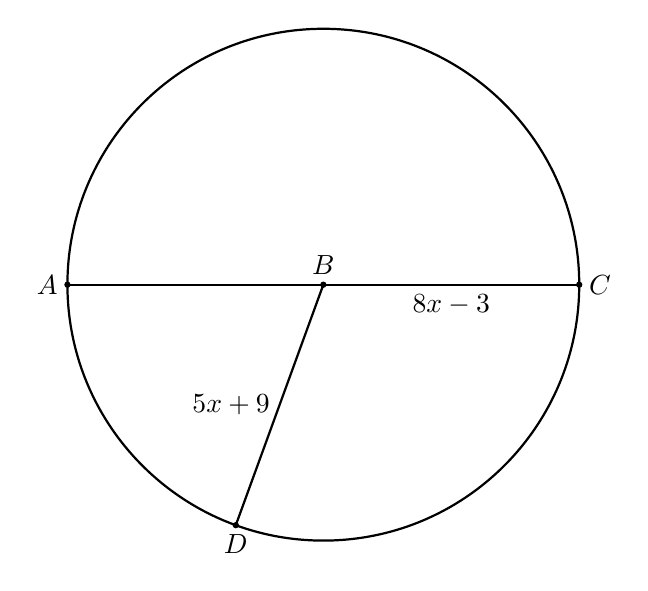
\begin{tikzpicture}[scale=0.65]
    \draw [thick] (0,0) circle [radius=5];
    \draw [-, thick] (-5,0)--(0,0)--(5,0);
    \draw [-, thick] (0,0)--(-110:5);
    \draw [fill] (-5,0) circle [radius=0.05] node[left]{$A$};
    \draw [fill] (0,0) circle [radius=0.05] node[above]{$B$};
    \draw [fill] (5,0) circle [radius=0.05] node[right]{$C$};
    \draw [fill] (-110:5) circle [radius=0.05] node[below]{$D$};
    \node at (-110:2.5)[left]{$5x+9$};
    \node at (2.5, 0)[below]{$8x-3$};
  \end{tikzpicture}
  \end{flushleft} \vspace{2cm}

\end{enumerate}
\end{document}
